\chapter{End-to-End Machine Learning Project\label{End-to-End Machine Learning Project}}
\section{Working with Real Data\label{Working with Real Data}}

When you are learning about Machine Learning, it is best to experiment with realworld data, not artificial datasets. Here are a few places you can look
to get data:
\begin{itemize}
\item Popular open data repositories
\begin{itemize}
\item \href{http://archive.ics.uci.edu/ml/index.php}{UC Irvine Machine Learning Repository}

\item \href{https://www.kaggle.com/datasets}{Kaggle datasets}

\item \href{https://registry.opendata.aws/}{Amazon's AWS datasets}
\end{itemize}

\item Meta portals (they list open data repositories)
\begin{itemize}
\item \href{http://dataportals.org/}{Data Portals}

\item \href{http://opendatamonitor.eu/}{OpenDataMonitor}

\item \href{https://data.nasdaq.com/}{Quandl}
\end{itemize}

\item Other pages listing many popular open data repositories
\begin{itemize}
\item \href{https://en.wikipedia.org/wiki/List_of_datasets_for_machine-learning_research}{Wikipedia’s list of Machine Learning datasets}

\item\href{https://www.quora.com/Where-can-I-find-large-datasets-open-to-the-public}{Quora.com}

\item\href{https://www.reddit.com/r/datasets/}{The datasets subreddit}
\end{itemize}
\end{itemize}

\section{Look at the Big Picture}
\subsection{Frame the Problem}
The first question to ask your boss is what exactly the business objective is. Building a
model is probably not the end goal. How does the company expect to use and benefit
from this model? Knowing the objective is important because it will determine how
you frame the problem, which algorithms you will select, which performance measure you will use to evaluate your model, and how much effort you will spend tweaking it.

Your boss answers that your model's output (a prediction of a district’s median housing price) will be fed to another Machine Learning system (see \autoref{A Machine Learning pipeline for real estate investments}), along
with many other signals\footnote{A piece of information fed to a Machine Learning system is often called a signal, in reference to Claude Shannon’s information theory, which he developed at Bell Labs to improve telecommunications. His theory: you
want a high signal-to-noise ratio.}.

\begin{figure}
\centering
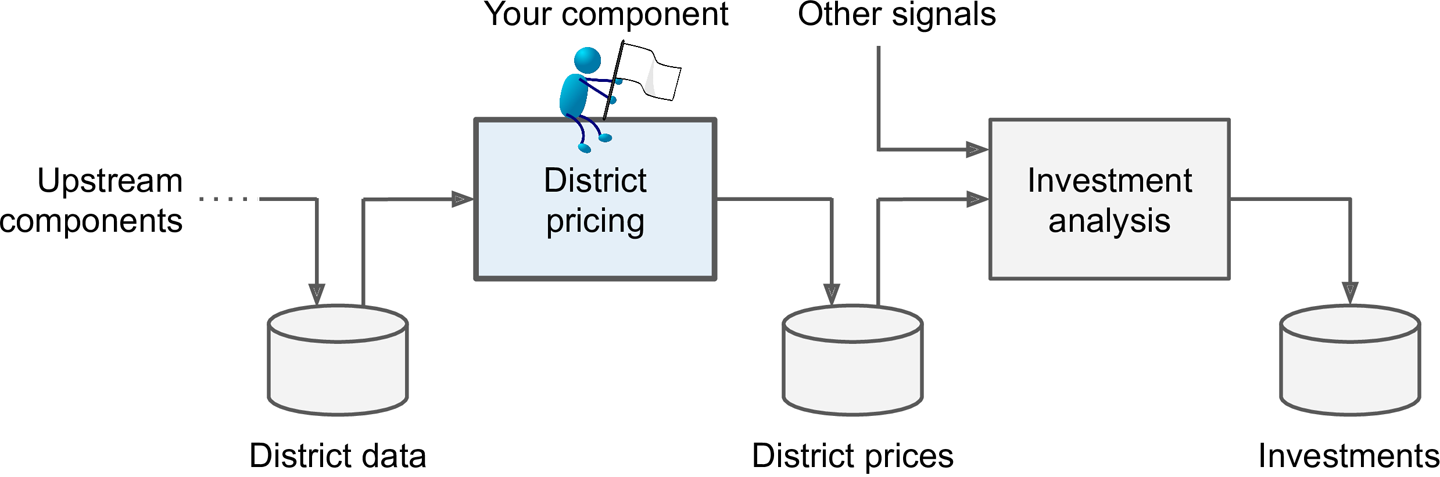
\includegraphics{img/A Machine Learning pipeline for real estate investments.png}
\caption{A Machine Learning pipeline for real estate investments}
\label{A Machine Learning pipeline for real estate investments}
\end{figure}
\explain{Pipelines}{
A sequence of data processing components is called a data pipeline. Pipelines are very
common in Machine Learning systems, since there is a lot of data to manipulate and
many data transformations to apply.

Components typically run asynchronously. Each component pulls in a large amount
of data, processes it, and spits out the result in another data store. Then, some time
later, the next component in the pipeline pulls this data and spits out its own output.
Each component is fairly self-contained: the interface between components is simply
the data store. This makes the system simple to grasp (with the help of a data flow
graph), and different teams can focus on different components. Moreover, if a component breaks down, the downstream components can often continue to run normally (at least for a while) by just using the last output from the broken component.
This makes the architecture quite robust.

On the other hand, a broken component can go unnoticed for some time if proper
monitoring is not implemented. The data gets stale and the overall system’s performance drops.
}

The next question to ask your boss is what the current solution looks like (if any).
The current situation will often give you a reference for performance

\textbf{Tips:}If the data were huge, you could either split your batch learning
work across multiple servers (using the MapReduce technique) or
use an online learning technique.

\subsection{Select a Performance Measure}
Your next step is to select a performance measure. A typical performance measure for
regression problems is the Root Mean Square Error (RMSE). It gives an idea of how
much error the system typically makes in its predictions, with a higher weight for
large errors. \autoref{RMSE} shows the mathematical formula to compute the RMSE.

\begin{equation}\label{RMSE}
RMSE(\mathbf{X}, h) = \sqrt{\frac{1}{m}\sum_{i=1}^m(h(x^{(i)})-y^{(i)})^2}
\end{equation}

\explain{Notations}{
This equation introduces several very common Machine Learning notations that we
will use throughout this book:
\begin{itemize}
\item $m$ is the number of instances in the dataset you are measuring the RMSE on.

\item $\mathbf{x}^{(i)}$ is a vector of all the feature values (excluding the label) of the $i^{th}$ instance in
the dataset, and $y^{(i)}$ is its label (the desired output value for that instance). e.g., 
\begin{align*}
\mathbf{x}^{(i)}&=\begin{bmatrix}
-118.29\\
33.91\\
1,416\\
38,372
\end{bmatrix}
\end{align*}


\item
$\mathbf{X}$ is a matrix containing all the feature values (excluding labels) of all instances in
the dataset. There is one row per instance, and the $i^{th}$ row is equal to the transpose of $\mathbf{x}^{(i)}$, noted $(\mathbf{x}^{(i)})^T$. e.g.,

\begin{align*}
\mathbf{x}^{(i)}&=\begin{bmatrix}
(\mathbf{x}^{(1)})^T\\
(\mathbf{x}^{(2)})^T\\
\vdots\\
(\mathbf{x}^{(m-1)})^T\\
(\mathbf{x}^{(m)})^T
\end{bmatrix}=\begin{bmatrix}
-118.29&33.91&1,416&38,372\\
\vdots&\vdots&\vdots&\vdots\\
\end{bmatrix}
\end{align*}
\item  $h$ is your system’s prediction function, also called a \emph{hypothesis}. When your system
is given an instance’s feature vector $\mathbf{x}^{(i)}$, it outputs a predicted value $\hat{y}^{(i)} = h(\mathbf{x}^{(i)})$ for that instance.

\item $RMSE(\mathbf{X}, h)$ is the cost function measured on the set of examples using your
hypothesis \emph{h}.

We use lowercase italic font for scalar values and function names, lowercase bold font for vectors, and uppercase bold font for
matrices.
\end{itemize}
}

Even though the RMSE is generally the preferred performance measure for regression
tasks, in some contexts you may prefer to use another function. For example, \textbf{suppose
that there are many outlier districts. In that case, you may consider using the mean
absolute error} (MAE, also called the average absolute deviation; see \autoref{MAE}):

\begin{equation}\label{MAE}
MAE(\mathbf{X}, h) = \frac{1}{m}\sum_{i=1}^m|h(x^{(i)})-y^{(i)}|
\end{equation}

Both the RMSE and the MAE are ways to measure the distance between two vectors:
the vector of predictions and the vector of target values. Various distance measures,
or \emph{norms}, are possible:

\begin{itemize}
\item
Computing the root of a sum of squares (RMSE) corresponds to the \emph{Euclidean
norm}: this is the notion of distance you are familiar with. It is also called the \emph{$l_2$
norm}, noted $||\cdot||_2$ (or just$||\cdot||$).
\item
Computing the sum of absolutes (MAE) corresponds to the \emph{$l_1$ norm}, noted $||\cdot||_1$.
This is sometimes called the \emph{Manhattan norm} because it measures the distance
between two points in a city if you can only travel along orthogonal city blocks.
\item More generally, the $l_k$ norm of a vector $v$ containing $n$ elements is defined as $||v||_k
= (|v_0|^k + |v_1|^k + \cdots + |v_n|^k)^{1/k}$. $l_0$ gives the number of nonzero elements in the vector, and $l_\infty$ gives the maximum absolute value in the vector.
\item \textbf{The higher the norm index, the more it focuses on large values and neglects small
ones.} This is why the RMSE is more sensitive to outliers than the MAE. But when
outliers are exponentially rare (like in a bell-shaped curve), the RMSE performs
very well and is generally preferred.
\end{itemize}

\subsection{Check the Assumptions}
Lastly, it is good practice to list and verify the assumptions that have been made so far
(by you or others); this can help you catch serious issues early on. For example, the
district prices that your system outputs are going to be fed into a downstream
Machine Learning system, and you assume that these prices are going to be used as
such. But what if the downstream system converts the prices into categories (e.g.,
“cheap,” “medium,” or “expensive”) and then uses those categories instead of the pri‐
ces themselves? In this case, getting the price perfectly right is not important at all;
your system just needs to get the category right. If that’s so, then the problem should
have been framed as a classification task, not a regression task. You don’t want to find
this out after working on a regression system for months.

\section{Get the Data}
The full Jupyter notebook is available at \url{https://github.com/JPL-JUNO/HOML}.
\subsection{Create the Workspace}
You will need to have Python installed. It is probably already installed on your
system. If not, you can get it at \url{https://www.python.org/}.

If you already have Jupyter running with all these modules installed,
you can safely skip to \nameref{Download the Data}.
\subsection{Download the Data\label{Download the Data}}

Having a function that downloads the data is useful in particular if the
data changes regularly: you can write a small script that uses the function to fetch the
latest data (or you can set up a scheduled job to do that automatically at regular intervals). Automating the process of fetching the data is also useful if you need to install
the dataset on multiple machines.

\subsection{Take a Quick Look at the Data Structure}
Let’s take a look at the five rows using the DataFrame’s \verb|sample(n=5)| method instead of \verb|head(n=5)|.

The \verb|info()| method is useful to get a quick description of the data, in particular the
total number of rows, each attribute’s type, and the number of nonnull values. Notice that the 
\verb|total_bedrooms| attribute has only 20,433 nonnull values, meaning that 207 districts are missing
this feature. We will need to take care of this later.

You can find out what cate‐
gories exist and how many districts belong to each category by using the
\verb|value_counts()| method:

\begin{minted}{python}
housing['ocean_proximity'].value_counts()
\end{minted}

The \verb|describe()| method shows a summary of the
numerical attributes. When with many columns, you can use \verb|transpose()| for best information.
\begin{minted}{python}
# housing.describe()
housing.describe().transpose()
\end{minted}

Another quick way to get a feel of the type of data you are dealing with is to plot a
histogram for each numerical attribute. A histogram shows the number of instances
(on the vertical axis) that have a given value range (on the horizontal axis). You can
either plot this one attribute at a time, or you can call the \verb|hist()| method on the whole dataset, and it will plot a histogram
for each numerical attribute (see \autoref{A histogram for each numerical attribute}):
\begin{minted}{python}
%matplotlib inline
import matplotlib.pyplot as plt
housing.hist(bins=50, figsize=(20, 15))
plt.show()
\end{minted}

\begin{pyc}
%matplotlib inline
import matplotlib.pyplot as plt
housing.hist(bins=50, figsize=(20, 15))
plt.show()
\end{pyc}

\begin{figure}
\centering
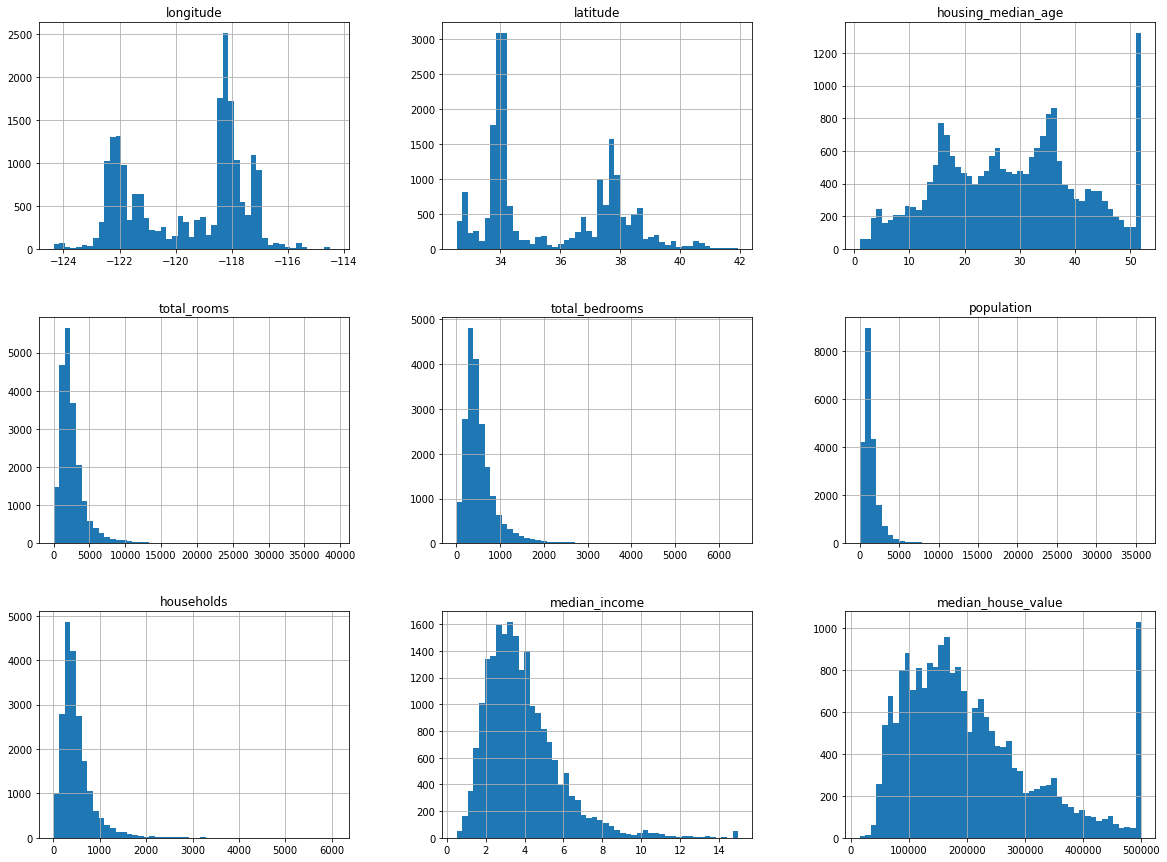
\includegraphics{img/codes/A histogram for each numerical attribute.png}
\caption{A histogram for each numerical attribute}
\label{A histogram for each numerical attribute}
\end{figure}

\notes{
The \texttt{hist()} method relies on Matplotlib, which in turn relies on a
user-specified graphical backend to draw on your screen. So before
you can plot anything, you need to specify which backend Matplotlib should use. The simplest option is to use Jupyter’s magic command \texttt{\%matplotlib inline}. This tells Jupyter to set up Matplotlib
so it uses Jupyter’s own backend. Plots are then rendered within the
notebook itself. Note that calling \texttt{show()} is optional in a Jupyter
notebook, as Jupyter will automatically display plots when a cell is
executed.
}

There are a few things you might notice in these histograms:
\begin{enumerate}
\item First, the median income attribute does not look like it is expressed in US dollars
(USD). After checking with the team that collected the data, you are told that the
data has been scaled and capped at 15 (actually, 15.0001) for higher median
incomes, and at 0.5 (actually, 0.4999) for lower median incomes. Working with preprocessed attributes is common in Machine Learning, and it is not necessarily a problem, but you should try to understand how the
data was computed.
\item
The housing median age and the median house value were also capped. The latter may be a serious problem since it is your target attribute (your labels). Your
Machine Learning algorithms may learn that prices never go beyond that limit.
You need to check with your client team (the team that will use your system’s output) to see if this is a problem or not. If they tell you that they need precise predictions even beyond \$500,000, then you have two options:
\begin{enumerate}
\item Collect proper labels for the districts whose labels were capped.
\item Remove those districts from the training set (and also from the test set, since
your system should not be evaluated poorly if it predicts values beyond
\$500,000).
\end{enumerate} 
\item These attributes have very different scales. We will discuss this later in this chapter, when we explore feature scaling.

\item Finally, many histograms are \emph{tail-heavy}: they extend much farther to the right of
the median than to the left. This may make it a bit harder for some Machine
Learning algorithms to detect patterns. We will try transforming these attributes
later on to have more bell-shaped distributions.
\end{enumerate}

\warning{Wait! Before you look at the data any further, you need to create a
test set, put it aside, and never look at it.}

\subsection{Create a Test Set}
It may sound strange to voluntarily set aside part of the data at this stage. After all,
you have only taken a quick glance at the data, and surely you should learn a whole
lot more about it before you decide what algorithms to use, right? This is true, but
your brain is an amazing pattern detection system, which means that it is highly
prone to overfitting: if you look at the test set, you may stumble upon some seemingly
interesting pattern in the test data that leads you to select a particular kind of
Machine Learning model. When you estimate the generalization error using the test
set, your estimate will be too optimistic, and you will launch a system that will not
perform as well as expected. This is called \emph{data snooping} bias.

Creating a test set is theoretically simple: pick some instances randomly, typically
20\% of the dataset (or less if your dataset is very large), and set them aside:
\begin{pyc}
import numpy as np
def split_train_test(data, test_ratio):
    shuffled_indices = np.random.permutation(len(data))
    test_set_size = int(len(data) * test_ratio)
    test_indices = shuffled_indices[: test_set_size]
    train_indices = shuffled_indices[test_set_size: ]
    return data.iloc[train_indices], data.iloc[test_indices]

train_set, test_set = split_train_test(housing, .2)
len(train_set), len(test_set)
# (16512, 4128)
\end{pyc}

Well, this works, but it is not perfect: if you run the program again, it will generate a different test set! Over time, you (or your Machine Learning algorithms) will get to
see the whole dataset, which is what you want to avoid.

One solution is to save the test set on the first run and then load it in subsequent
runs. \textbf{Another option is to set the random number generator’s seed} (e.g., with \verb|np.random.seed(42)|)\footnote{You will often see people set the random seed to 42. This number has no special property, other than to be the
Answer to the Ultimate Question of Life, the Universe, and Everything.} before calling \verb|np.random.permutation()| so that it always generates
the same shuffled indices.

But both these solutions will break the next time you fetch an updated dataset. To
have a stable train/test split even after updating the dataset, a common solution is to
use each instance’s identifier to decide whether or not it should go in the test set
(assuming instances have a unique and immutable identifier). For example, you could
compute a hash of each instance’s identifier and put that instance in the test set if the
hash is lower than or equal to 20\% of the maximum hash value. This ensures that the
test set will remain consistent across multiple runs, even if you refresh the dataset.
The new test set will contain 20\% of the new instances, but it will not contain any
instance that was previously in the training set.

Here is a possible implementation(more about \href{https://baike.baidu.com/item/CRC32/7460858}{crc32}):
\begin{pyc}
from zlib import crc32
def test_set_check(identifier, test_ratio):
    return crc32(np.int64(identifier)) & 0xffffffff < test_ratio * 2 ** 32

def split_train_test_by_id(data, test_ratio, id_column):
    ids = data[id_column]
    in_test_set = ids.apply(lambda id_: test_set_check(id_, test_ratio))
    return data.loc[~in_test_set], data.loc[in_test_set]

housing_with_id = housing.reset_index()
train_set, test_set = split_train_test_by_id(housing_with_id, .2, 'index')
len(train_set), len(test_set)
# (16512, 4128)
\end{pyc}

If you use the row index as a unique identifier, you need to make sure that new data
gets appended to the end of the dataset and that no row ever gets deleted. If this is not
possible, then \textbf{you can try to use the most stable features to build a unique identifier}. For example, a district’s latitude and longitude are guaranteed to be stable for a few
million years, so you could combine them into an ID like so:

\begin{pyc}
housing_with_id['id'] = housing['longitude'] * 1000 + housing['latitude']
train_set, test_set = split_train_test_by_id(housing_with_id, .2, 'id')
len(train_set), len(test_set)
# (16322, 4318)
\end{pyc}

Scikit-Learn provides a few functions to split datasets into multiple subsets in various
ways. The simplest function is \verb|train_test_split()|. First, there is a \verb|random_state| parameter that allows you to set the random generator
seed. Second, you can pass it multiple datasets with an identical number of rows, and
it will split them on the same indices (this is very useful, for example, if you have a
separate DataFrame for labels):
\begin{pyc}
from sklearn.model_selection import train_test_split
train_set, test_set = train_test_split(housing, test_size=.2, random_state=42)
len(train_set), len(test_set)
# (16512, 4128)
\end{pyc}

So far we have considered purely random sampling methods. This is generally fine if
your dataset is large enough (especially relative to the number of attributes), but if it
is not, you \textbf{run the risk of introducing a significant sampling bias}. When a survey
company decides to call 1,000 people to ask them a few questions, they don’t just pick
1,000 people randomly in a phone book. They try to ensure that these 1,000 people
are representative of the whole population. For example, the US population is 51.3\%
females and 48.7\% males, so a well-conducted survey in the US would try to maintain
this ratio in the sample: 513 female and 487 male. This is called stratified sampling:
the population is divided into homogeneous subgroups called strata, and the right
number of instances are sampled from each stratum to guarantee that the test set is
representative of the overall population. If the people running the survey used purely
random sampling, there would be about a 11.29\% chance of sampling a skewed test set that was either less than 49\% female or more than 54\% female(Why see \href{https://github.com/JPL-JUNO/HOML/blob/main/chapter/chapter2.ipynb}{Notebook chapter2}). Either way, the survey results would be significantly biased.

Suppose you chatted with experts who told you that the median income is a very
important attribute to predict median housing prices. You may want to ensure that
the test set is representative of the various categories of incomes in the whole dataset. It is important to have a sufficient number of instances in your dataset for each stratum, or else the estimate
of a stratum’s importance may be biased. \textbf{This means that you should not have too
many strata, and each stratum should be large enough.}

\begin{pyc}
housing['income_cat'] = pd.cut(housing['median_income'],
                               bins=[0, 1.5, 3.0, 4.5, 6, np.inf], 
                               labels=[1, 2, 3, 4, 5])
housing['income_cat'].hist()
\end{pyc}
\begin{figure}
\centering
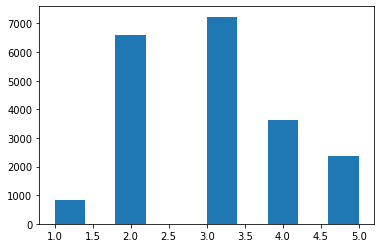
\includegraphics{img/codes/Histogram of income categories.png}
\caption{Histogram of income categories}
\label{Histogram of income categories}
\end{figure}
Now you are ready to do stratified sampling based on the income category. For this
you can use Scikit-Learn’s \verb|StratifiedShuffleSplit|(more about \href{https://scikit-learn.org/stable/modules/cross_validation.html}{StratifiedShuffleSplit}) class:

\begin{pyc}
from sklearn.model_selection import StratifiedShuffleSplit
split = StratifiedShuffleSplit(n_splits=1, test_size=.2, random_state=42)
for train_index, test_index in split.split(housing, housing['income_cat']):
    strat_train_set = housing.loc[train_index]
    strat_test_set = housing.loc[test_index]
strat_test_set['income_cat'].value_counts() / len(strat_test_set)
\end{pyc}

 As you can see, the test set generated using stratified sampling has
income category proportions almost identical to those in the full dataset, whereas the
test set generated using purely random sampling is skewed(for more see \href{https://github.com/JPL-JUNO/HOML/blob/main/chapter/chapter2.ipynb}{Notebook chapter2}).

We spent quite a bit of time on test set generation for a good reason: this is an often
neglected but critical part of a Machine Learning project. Moreover, many of these
ideas will be useful later when we discuss cross-validation.
